\chapter{Intrinsic Channel Properties and Scattering Mechanisms}\label{chap:results}
Developing low resistance two-dimensional/two-dimensional (2D/2D) ohmic contacts opens up possibility to study the intrinsic properties of \acp{TMD} and quantum physics. In particular, quantum phenomena inherent to \acp{2DEG} and \acp{2DHG} such as the \ac{IQHE} and \ac{SdH} oscillations can be explored in high mobility monolayer and few-layer \acp{TMD} \cite{Cui_NatureNano2015}. In addition to quantum transport properties and quantum effects in monolayer and few-layer \acp{TMD} the study of mobility and its corresponding temperature dependence can be used to understand the multiple scattering mechanisms present \cite{Kaasbjerg_PhysRevB2012}. These study of both electron and hole transport mechanisms is important due to the fact that high-performance $p$-type and $n$-type transistors are necessary for complimentary digital applications. 

\section{$p$-type \ch{WSe2} Semiconductor Contact Resistance}\label{sec:pWSe2_contacts}
One of the major challenges that still remains in fabricating devices to study intrinsic channel properties and scattering mechanisms is developing high quality $p$-type \ch{WSe2} devices. This is due to the fact that the metal/\ch{WSe2} (or \ch{MoS2}) interface is obstructed by a large \ac{SB} formed by the Fermi level pinning close to the conduction band of the \ch{WSe2} \cite{Chuang_NanoLett2014,Das_NanoLett2012}. \\ \\

\noindent In order to fabricate high quality $p$-type \ch{WSe2} devices, one aspect that must be addressed is how doping affects the \ac{SBH}. In particular, it is important to determine how doping can improve the 2D/2D contacts in devices. To address this issue of contact resistance several devices were fabricated and characterized in order to determine the contact resistance. Using the \ac{TLM} several \ch{WSe2} devices were made with electrodes spaced at varying lengths from the source electrode. 
\begin{figure}[ht]
	\centering
	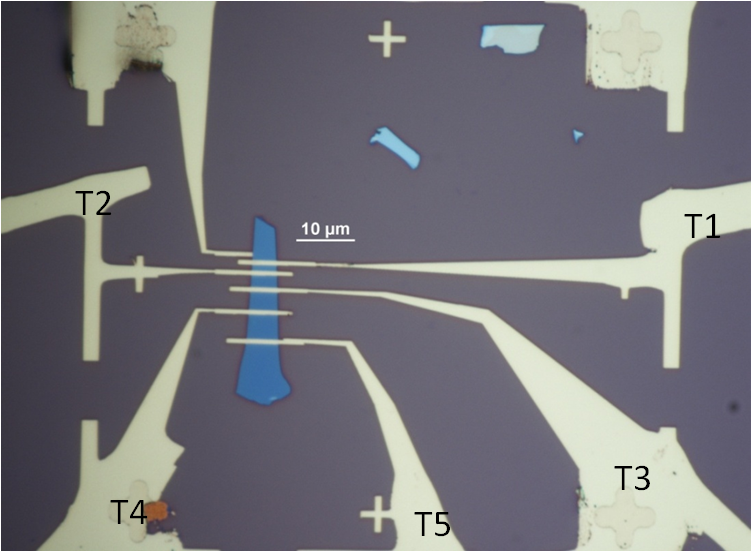
\includegraphics[height=5cm,width=7cm]{figs/results/transmission_line/transmission_device_pic_5-5_21_10232015_no1}
	\caption[Transmission line $0.05\%$ \ch{Nb} doped \ch{WSe2} channel device]{$0.05\%$ \ch{Nb} doped \ch{WSe2} channel transmission lines with corresponding channel lengths and widths of $L_{12} = 1.04\unita{\mu m}$ $W_{12} = 4.42\unita{\mu m}$, $L_{23} = 2.04\unita{\mu m}$, $W_{23} = 4.47\unita{\mu m}$, $L_{34} = 3.09\unita{\mu m}$, $W_{34} = 4.90\unita{\mu m}$, $W_{45} = 5.15\unita{\mu m}$, and $L_{45} = 4.27\unita{\mu m}$.}
	\label{fig:transmission_device_10232015_no1}
\end{figure}
Fig.~\ref{fig:transmission_device_10232015_no1} illustrates an example of a transmission line device that was used to characterize the contact resistance. The device shown has a $0.05\%$ \ch{Nb} doped \ch{WSe2} channel. The resistance in general is given by
\begin{equation}\label{eq:resistance_formula}
	R = \frac{\rho}{A} l,
\end{equation}
where, in this case, it is assumed that the resistivity $\rho$ and the area $A$ are constant throughout the device \cite{Schroder_Semiconductor2006}. The resistance $R$ is then proportional to the length $l$. By determining the resistance as a function of length one can determine the contact resistance of the device. The total resistance of the device is given by
\begin{equation}\label{eq:resistance_total}
	R = R_\mathrm{c} + R_\mathrm{ch},
\end{equation}
where $R_\mathrm{c}$ and $R_\mathrm{ch}$ are the contact and channel resistances, respectively \cite{Schroder_Semiconductor2006}. Thus by finding the resistance from the gradient of an I-V characteristic curve, one can apply the logic from eqs.~\ref{eq:resistance_formula} and \ref{eq:resistance_total} to find the contact resistance.
\begin{figure}[ht]
	\centering
	\subfloat[Caption]{
		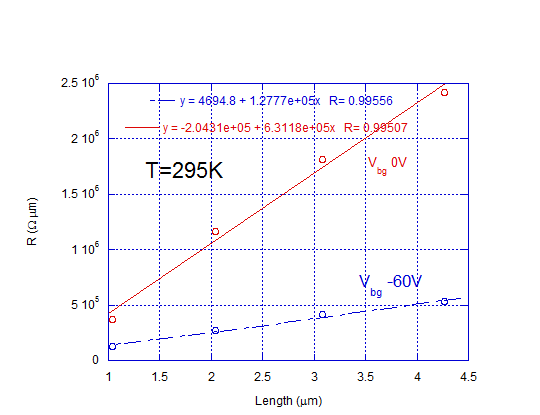
\includegraphics[height=3.5cm,width=4.25cm]{figs/results/transmission_line/transmission_resistance_plot_pic_5-5_21_10232015_no1}
		\label{fig:tlm_resistance1}
	}
	\qquad
	\subfloat[Caption]{
		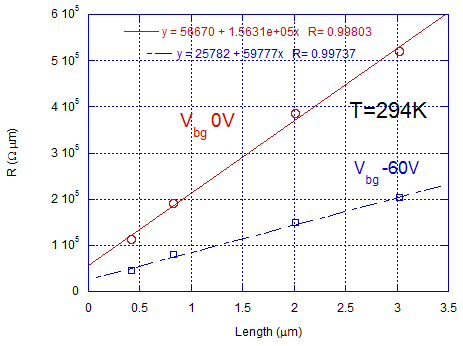
\includegraphics[height=3.5cm,width=4.25cm]{figs/results/transmission_line/transmission_resistance_plot_pic_56_21_10232015_no2}
		\label{fig:tlm_resistance2}
	}
	\qquad
	\subfloat[Caption]{
		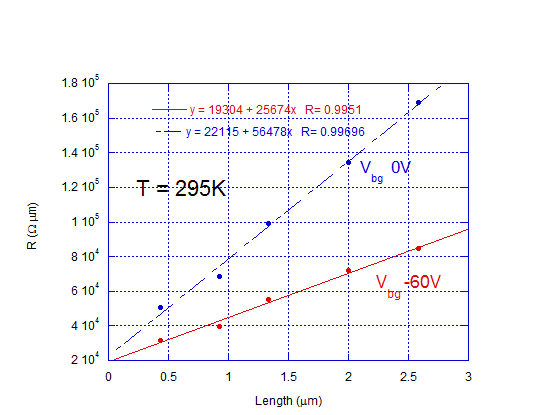
\includegraphics[height=3.5cm,width=4.25cm]{figs/results/transmission_line/transmission_resistance_plot_pic_-66_21_11182015_no2}
		\label{fig:tlm_resistance3}
	}
	\caption[Contact resistance of $0.05\%$ \ch{Nb} doped \ch{WSe2} channel device]{Main Caption}
	\label{fig:tlm_reistance_measurement}
\end{figure}
Using this method the resistance as a function of length is shown in figs.~\subref*{fig:tlm_resistance1}, \subref*{fig:tlm_resistance2}, and \subref*{fig:tlm_resistance3} for both $V_{bg} = 0\unita{V}$ and $V_{bg} = -60\unita{V}$. From these figures one can interpret the contact resistance of the device as the intercept value with the value for $V_{bg} = -60\unita{V}$ being the more accurate of the two (WHY IS THIS TRUE?). The resulting contact resistances are summarized in table~\ref{table:contact_summary}.
\begin{table}[ht]
	\centering
	\begin{threeparttable}
		\begin{tabular}{c c c c}
			\hline\hline
			$L_\mathrm{min}$ & $L_\mathrm{max}$ & $R_\mathrm{c}(\unita{k\Omega\cdot\mu m})$ at $V_{bg} = 0\unita{V}$ & $R_\mathrm{c}(\unita{k\Omega\cdot\mu m})$ at $V_{bg} = -60\unita{V}$ \\ [0.5ex]
			\hline
			$1.04\unita{\mu m}$ & $4.27\unita{\mu m}$ & $204$\tnote{a} & $4.70$\tnote{a}\\
			$0.42\unita{\mu m}$ & $3.02\unita{\mu m}$ & $56.7$\tnote{b} & $25.8$\tnote{b}\\
			$0.43\unita{\mu m}$ & $2.58\unita{\mu m}$ & $22.1$\tnote{c} & $19.3$\tnote{c}\\ [1ex]
			\hline
		\end{tabular}
		\begin{tablenotes}
			\item[a] Length and resistance values from fig.~\subref*{fig:tlm_resistance1}.
			\item[b] Length and resistance values from fig.~\subref*{fig:tlm_resistance2}.
			\item[c] Length and resistance values from fig.~\subref*{fig:tlm_resistance3}.
		\end{tablenotes}
	\caption[Summary of contact resistances for $0.05\%$ \ch{Nb} doped \ch{WSe2} channel]{Main Caption}
	\label{table:contact_summary}
	\end{threeparttable}
\end{table}

\section{$p$-type \ch{WSe2} Semiconductor Intrinsic Channel Properties}\label{sec:pWSe2_intrinsic_properties}
In addition to knowing the how doping can be used to lower the \acs{SBH}, doping also affects the intrinsic channel properties. To study how these properties are effected several measurements were taken. First, Hall bar devices were fabricated. These devices were similar to those used in sec.~\ref{sec:pWSe2_contacts}, the channel was doped with the same amount of \ch{Nb}. The only differing aspect of these devices was the electrode design. Fig.~\ref{fig:hall_bar_device1} shows an example of one such Hall bar device. 
\begin{figure}[ht]
	\centering
	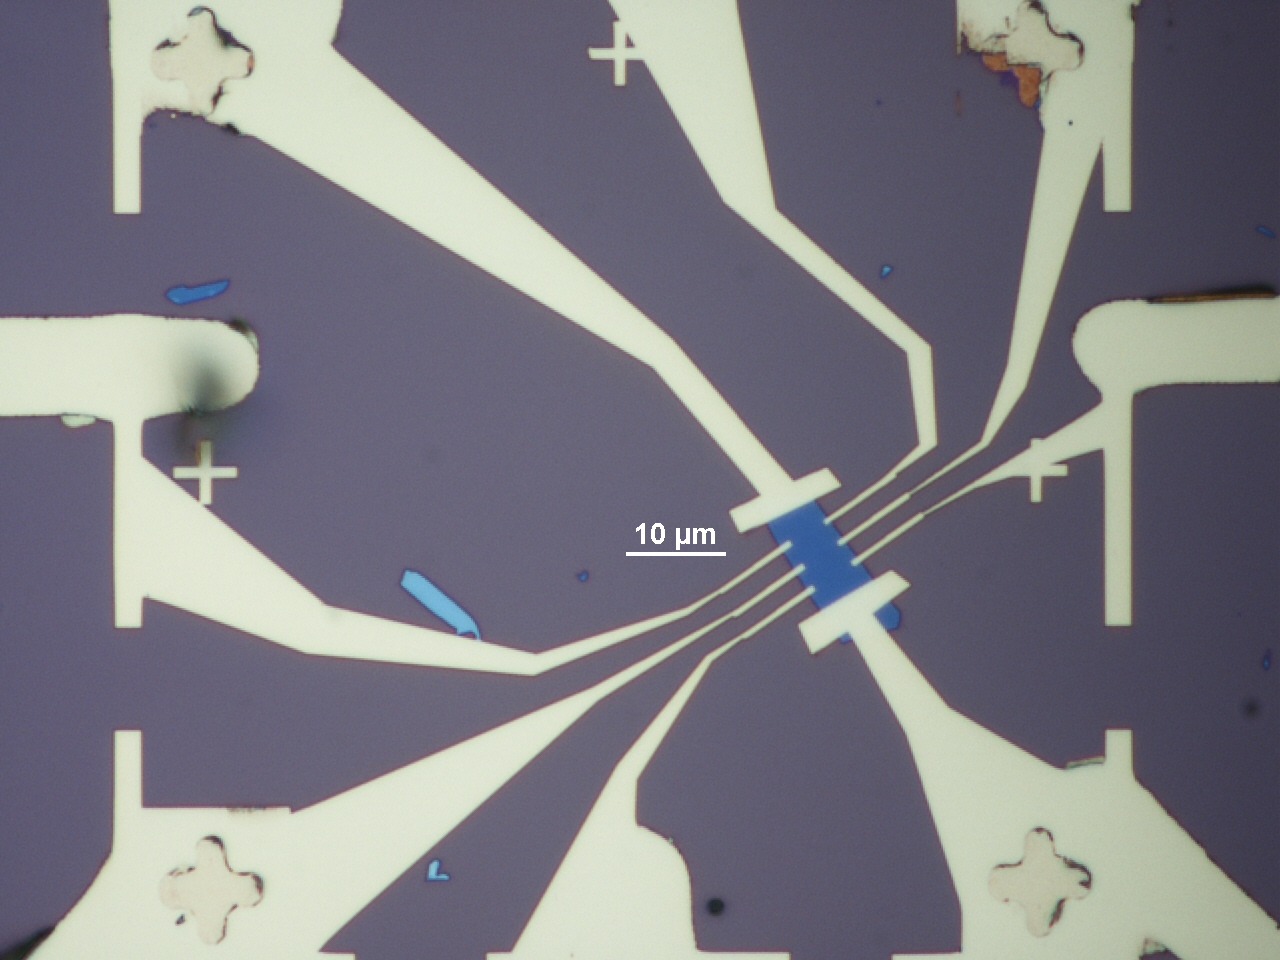
\includegraphics[height=5cm,width=7cm]{figs/results/hall_bar_doped_channel/hall_bar_device_pic_11192015_no1}
	\caption[Hall bar device with $0.05\%$ \ch{Nb} doped \ch{WSe2} channel]{Hall bar device with $0.05\%$ \ch{Nb} doped \ch{WSe2} channel. Sample thickness is $7.74\unita{nm}$ with an average width $W_\mathrm{avg}=5.74\unita{\mu m}$.}
	\label{fig:hall_bar_device1}
\end{figure}